\documentclass[12pt,a4paper]{standalone}
\usepackage[utf8]{inputenc}
\usepackage{amsmath}
\usepackage{amsfonts}
\usepackage{amssymb}
\usepackage{graphicx}
\newcommand*{\eps}{0.05}
\newcommand*{\Real}{\,\text{Re}}
\usepackage{tikz}
\usepackage{pgfplots}
\pgfplotsset{compat=newest}
\usetikzlibrary{decorations.markings}
\begin{document}
	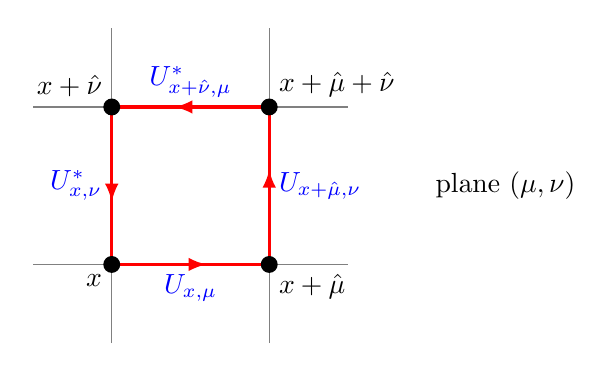
\begin{tikzpicture}
		\tikzset{middlearrow/.style={decoration={markings,mark= at position 0.6 with {\arrow{#1}} ,},postaction={decorate}}};
		\draw[step=2cm,color=gray] (-1,-1) grid (3,3);
		\draw[middlearrow={latex}, very thick,red] (0,0) --(2,0);
		\draw[middlearrow={latex}, very thick,red] (2,0)--(2,2);
		\draw[middlearrow={latex}, very thick,red] (2,2)--(0,2);
		\draw[middlearrow={latex}, very thick,red] (0,2)--(0,0);
		\filldraw[black] (0,0) circle(0.1);
		\filldraw[black] (2,0) circle(0.1);
		\filldraw[black] (2,2) circle(0.1);
		\filldraw[black] (0,2) circle(0.1);
		\draw[] (0,0) node[below left] {$x$};
		\draw[] (2,0) node[below right] {$x+\hat\mu$};
		\draw[] (0,2) node[above left] {$x+\hat\nu$};
		\draw[] (2,2) node[above right] {$x+\hat\mu+\hat\nu$};
		
		\draw[] (5,1) node[] {plane $(\mu,\nu$)};
		
		\draw[blue] (1,0) node[below] {$U_{x,\mu}$};
		\draw[blue] (2,1) node[right] {$U_{x+\hat\mu,\nu}$};	
		\draw[blue] (1,2) node[above] {$U^*_{x+\hat\nu,\mu}$};
		\draw[blue] (0,1) node[left] {$U^*_{x,\nu}$};
			
	\end{tikzpicture}
\end{document}